\documentclass[12pt,draftclsnofoot,journal,onecolumn]{IEEEtran}
\usepackage{amsfonts}
\usepackage{amsmath,amssymb}
\usepackage{acronym}  % make an acronym
\usepackage{algorithm}
\usepackage{algorithmic}
\usepackage{balance}
\usepackage{bm}
\usepackage{bbm}
\usepackage{booktabs}
\usepackage{color, soul}
\usepackage{cite}
\usepackage{flushend}
\usepackage{graphicx}
\usepackage{indentfirst}
\usepackage{setspace}
\usepackage{tikz}
\usetikzlibrary{arrows}
\usepackage{subfigure}
\usepackage[amsmath,thmmarks]{ntheorem}
\usepackage{theorem}
% Enable Hyper-references.
\usepackage{hyperref}
\hypersetup{hidelinks, 
colorlinks=true,
allcolors=black,
pdfstartview=Fit,
breaklinks=true}

\newtheorem{theorem}{\bf Theorem}
\newtheorem{proposition}{\bf Proposition}
\newtheorem{lemma}{\bf Lemma}
\newtheorem{definition}{Definition}
\newtheorem{remark}{\bf Remark}

\theoremheaderfont{~~~\it}\theorembodyfont{\upshape}%
\theoremstyle{nonumberplain}
\theoremseparator{}
\theoremsymbol{\rule{1ex}{1ex}}
\newtheorem{proof}{Proof:}
\acrodef{EAR}[EAR]{element activation ratio}
\acrodef{SNR}[SNR]{signal-to-noise ratio}
\acrodef{TC}[TC]{transmission coefficients}
\acrodef{US-RIS}[US-RIS]{user-side RIS}
\acrodef{BSS-RIS}[BSS-RIS]{base-station-side RIS}
\acrodef{DoF}[DoF]{degree of freedom}
\acrodef{FPGA}[FPGA]{field programmable gate array}
\acrodef{RF}[RF]{radio-frequency}
\acrodef{RIS}[RIS]{reconfigurable intelligent surfaces}
\acrodef{UE}[UE]{user equipment}
\acrodef{BS}[BS]{base station}
\acrodef{DL}[DL]{downlink}
\acrodef{TA}[TA]{transmit antenna}
\acrodef{RA}[RA]{receive antenna}
\acrodef{LoS}[LoS]{line-of-sight}
\acrodef{UL-TBF}[UL-TBF]{uplink transmit beamforming}
\acrodef{TPS}[TPS]{transmit phase shifter}
\acrodef{RC}[RC]{receiver combining}
\acrodef{AWGN}[AWGN]{additive white Gaussian noise}
\acrodef{DFT}[DFT]{discrete Fourier transform}
\acrodef{IRF}[IRF]{interferential random field}

\def \H {^H}
\def \opt {^{\text{opt}}}
\def \v {\bm v}
\def \w {\bm w}
\def \g {\bm g}
\def \f {\bm f}
\def \T {\bm \Theta}
\def \t {\bm \theta}
\def \x {\bm \xi}
\def \Pmax {P_{\text{max}}}
\def \ml {multi-layer }
\def \tb {transmit beamformer }
\def \sl {single-layer }
\def \diag {\text{diag}}
\def \opt {^{\text{opt}}}
\def \exp {\text{exp}}
\def \arg {\text{arg}}
\def \CN {\mathcal{CN}}
\def \VM {\mathcal{VM}}
\def \re {\rm Re}
\def \nc {\mathcal{NC}}

\newcommand{\RNum}[1]{\uppercase\expandafter{\romannumeral #1\relax}}
\renewcommand{\algorithmicrequire}{\textbf{Input:}}   %Use Input in the format of Algorithm
\renewcommand{\algorithmicensure}{\textbf{Output:}}  %UseOutput in the format of Algorithm
\ifCLASSINFOpdf
\else
\fi
\hyphenation{op-tical net-works semi-conduc-tor}
\begin{document}
\title{Sensing RIS}
\author{{Jieao Zhu, Kunzan Liu, Zhongzhichao Wan, and Linglong Dai
\vspace*{-1em}}
\thanks{Beijing National Research Center for Information Science and Technology (BNRist)}
%\thanks{Corresponding author: Linglong Dai.}
}

\maketitle

\begin{abstract}
xxx
\end{abstract}

\begin{IEEEkeywords}
xxx
\end{IEEEkeywords}
\section{Introduction}
    Now we introduce a new flavor of channel estimation and beamforming techniques in \ac{RIS}-aided wireless communication systems. When equipped with a Sensing \ac{RIS} \cite{ma2020smartsensing}, we can obtain CSI directly from the \ac{RIS} power sensors, and immediately calculate the beamforming phases for each \ac{RIS} element.

    There are three most significant benefits for using a Sensing-RIS system:
    \begin{itemize}
        \item The \ac{IRF} generated by the BS and UE makes it possible to obtain CSI within only one pilot slot. Thus, the pilot cost is reduced to $\mathcal{O}(1)$.
        \item After measuring the \ac{IRF}, the optimal phase for each \ac{RIS} element can be calculated within $\mathcal{O}(1)$ time.
        \item All the CSI acquisition and beamforming can be done directly at the \ac{RIS}, making channel feedback unnecessary.
    \end{itemize}

\section{System Model}  \label{System Model}
    In this section, we will first specify the channel model of the RIS-assisted MISO system. Then, the basic models, notations, and properties of the \ac{IRF} will be introduced.

    \subsection{RIS-Aided MISO System}  \label{MISO case}
        We consider the situation where a single-antenna user is served by an $M$-antenna BS and an $N$-element \ac{RIS}. The RIS phase-shift matrix is represented by
        \begin{equation}
            \label{RIS}
            \bm \Theta = \diag \left(\bm \theta\right )=\diag \left(\left[\theta_{1},\cdots ,\theta_{N}\right]\right),
        \end{equation}
        where $\theta_i, 1\leq i \leq N$ denotes the phase-shift coefficient of the $i$-th \ac{RIS} element, satisfying $\lvert \theta_i\rvert=1$. The UE-received symbol is then given by 
        \begin{equation}
            \label{Signal model}
            y=\bm f^{H} \bm\Theta \bm G \bm w s+z,
        \end{equation}
        where $\bm f\in \mathbb C ^{N\times 1}$ and $\bm G \in \mathbb C^{N\times M}$ denote the channel from the \ac{RIS} to the user and the channel from the BS to the \ac{RIS}, respectively; $\bm w\in \mathbb C^{M\times 1}$ denotes the beamforming vector at the transmitter BS, with $\left\Vert \bm w\right \Vert_{2}^{2}\leq P$; The letter $s$ denotes the normalized transmitted symbol; $z\sim \mathcal{CN}\left(0,\sigma_{z}^{2}\right)$ denotes the \ac{AWGN} introduced at the receiver user.
        In this paper, we assume that the \ac{BS} and \ac{RIS} are fixed. With fixed positions of the \ac{BS} and the \ac{RIS}, the optimal beamforming vector is expressed as 
        \begin{equation}
            \label{fixed w}
            \bm w=\sqrt{P_{\rm BS}}\bm a\left(\alpha\right),
        \end{equation}
        where $\alpha$ is the wave departure angle of the BS antenna array, and $P_{\rm BS}$ is the transmit power of the BS, measured in Watts. 

The SNR maximization problem for the receiver user can be formulated as
\begin{subequations}
\label{optimization}
\begin{align}
\label{objective}
\max_{\bm \Theta}~~&\text{SNR}=\frac{1}{\sigma_{z}^{2}}
\left\vert
\bm f^{H}\bm \Theta\bm G\bm w \right\vert^{2},\\
\label{constraint}
~~~~~\text{s.t.~~~}&\left\vert\theta_{n}\right\vert=1,~\forall n.
\end{align}
\end{subequations}

The optimal phase-shift for the $n$-th RIS element can be obtained as
\begin{equation}
\label{optimal RIS}
\theta_{n}\opt = \exp\left(-{\rm j} \arg\left(f_{n}^{*}\bm g_{n}^{T}\bm w\right)\right),~\forall n,
\end{equation}
where $\bm G = \left[\bm g_{1}, \cdots, \bm g_{N}\right]^{T}$.

\subsection{Traditional Channel Estimation Conventions}
    Traditional channel estimation requires the UE to be the pilot transmitter. The signal model is 
    \begin{equation}
        {\bm y}_{{\rm BS}, p} = {\bm G}^{T} {\rm diag}({\bm f}^{*}) {\bm \theta}_p x+n, 
    \end{equation}
    where ${\bm \theta}_p \in \mathbb{C}^{N\times 1}$ is the $p$-th RIS phase vector, and ${\bm y}_{{\rm BS}, p}$ is the $p$-th  BS received vector. The RIS phase vectors ${\bm \theta}_p$ is designed to be the first $P$ columns of the DFT matrix. After gathering the $P$ received vectors during $P$ consecutive pilot slots, assuming $x=1$, the matrix identity is expressed as 
    \begin{equation}
        {\bm Y}_{\rm BS}={\bm G}^{T} {\rm diag}({\bm f}^{*}) {\bm \Theta} + {\bm Z}, 
        \label{eqn:MMSE_CE}
    \end{equation} 
    where ${\bm Z}\in \mathbb{C}^{M\times P}$ and each element ${\bm Z}_{i,j}\sim \CN(0,\sigma^2)$, $\sigma^2=-174{\rm dBm/Hz}$. 
    Substituting ${\bm \Theta} = {\bm F}_{N,K}$ into \eqref{eqn:MMSE_CE} and denoting $\hat{\bm H} = {\bm G}^{\rm T}{\rm diag}({\bm f}^{*})$, then the MMSE channel estimation problem can be re-stated as 
    \begin{equation}
        \hat{\bm H} = \arg\max_{\bm H} \lVert {\bm Y}_{\rm BS} - {\bm H} {\bm F}_{N,K}\rVert_{F}^2,
    \end{equation}
    which is a least-square problem, and we know that this system is solved by 
    \begin{equation}
        \hat{\bm H} = \frac{1}{P}{\bm Y}{\bm F}_{N,K}^{H}.
    \end{equation}
    After obtaining $\hat{\bm H}$, we can optimize for ${\bm w}$ and ${\bm \theta}$ by iterative optimization.

\section{Channel Estimation with Interference Random Fields}
Interference field at the $n$-th RIS element, with transmitted symbol $s=1$:
\begin{equation}
\label{interference}
E_{n}(t)=\bm g_{n}^{T}\bm w+f_{n}^{*}e^{{\rm j}\psi (t)}+v(t).
\end{equation}

Define $\alpha = \left\vert\bm g_{n}^{T}\bm w\right\vert$ and $\beta = \left\vert f_{n}^{*}\right \vert$, and define the phase to be measured as $\varphi = \arg\left(f_{n}^{*}\right)-\arg\left(\bm g_{n}^{T}\bm w\right)$.
Then, the power of interference field can be written as
\begin{equation}
\label{Power of Interference}
\begin{aligned}
P(t)&=A \left| E_{n} (t)\right |^{2}+\zeta\\
&=\underbrace{A\left[\alpha^{2}+\beta^{2}+2\alpha\beta\cos\left(\psi(t)+\varphi\right)\right]}_{\text{Sensor detection signal}}\\
&~~~+\underbrace{2A\text{Re}\left\{\left(\alpha+\beta e^{j\left(\psi(t)+\varphi\right)}\right)v'^{*}(t)\right\}+A\left|v'(t)\right|^{2}+\zeta}_{\text{Noise}},\\
\end{aligned}
\end{equation}
where $v'\overset{\text{d}}{=}v\sim\mathcal{CN}\left(0,\sigma_{v}^{2}\right)$.

To estimate the phase $\varphi$, we need enough observations from the sensor detection signal. For simplicity and without loss of generality, let us assume $\psi(t)=\omega t$ and $\omega=\frac{2\pi}{T_{s}}$. Assume furthermore that $L$ observations $P[l]=P(t_{l})$ at time 
\begin{equation}
\label{observation time}
t_{l}=\frac{l}{L}T_{s},~\forall l\in \left\{0,\cdots ,L-1\right\}
\end{equation}
are used for estimation.
\subsection{LS method}
Apply $L$-point \ac{DFT} to the observed sensor detection signals $P[1],\cdots ,P[L]$, we have
\begin{equation}
\label{DFT}
p[l']=\sum\nolimits_{l=0}^{L-1}P[l]e^{-j\frac{2\pi}{L}ll'},~\forall l'\in [L].
\end{equation}
Specifically, we have
\begin{equation}
\label{DFT l=1}
p[1]=\sum\nolimits_{l=0}^{L-1}A\left[\alpha^{2}+\beta^{2}+2\alpha\beta\cos\left(\frac{2\pi}{L}l+\varphi\right)\right]e^{-j\frac{2\pi}{L}l}=\frac{A}{2}e^{j\varphi}.
\end{equation}
Then, the phase $\varphi$ can be estimated as
\begin{equation}
\label{LS estimate result}
\hat{\varphi}=\arg\left(\frac{2p[1]}{A}\right) = \arg\left(p[1]\right).
\end{equation}

%% zja working below
\subsection{ML method}
    Suppose the noise field $v'(t)=v'_R(t) + jv'_I(t)\sim \mathcal{CN}(0, \sigma_v^2)$, and the noise of the power sensor is $\zeta \sim \mathcal{N}(0, \sigma_{\zeta}^2)$. Then the distribution of $s(t) := A\left|E_n(t)\right|^2$ is a noncentral chi-squared distribution with degrees of freedom $k=2$, and mean values $\mu_{n,R}, \mu_{n,I}$ given by
    \begin{equation}
        \begin{aligned}
        \mu_{n,R} & = \alpha + \beta \cos(\psi(t)+\varphi),    \\ 
        \mu_{n,I} & = \beta \sin(\psi(t)+\varphi).   \\
        \end{aligned}
    \end{equation}
    Thus, the output of the power sensor is 
    \begin{equation}
        P(t)  = A\left((v'_{R} + \mu_{n,R})^2 + (v'_{I} + \mu_{n,I})^2 \right)+ \zeta 
        \label{eqn:sensor power}
    \end{equation}
    By defining the noncentral parameter $\lambda(t)$ as
    \begin{equation}
        \lambda(t)  = A(\mu_{n,R}^2 + \mu_{n,I}^2) = A\left[\alpha^{2}+\beta^{2}+2\alpha\beta\cos\left(\psi(t)+\varphi\right)\right],
    \end{equation}
    then the p.d.f of $s(t) := P(t)-\zeta$ is given by the zeroth-order modified Bessel function
    \begin{equation}
        f_{s(t)}(x) = \frac{1}{A\sigma_{v}^2} \exp\left(-\frac{x+\lambda(t)}{A\sigma_v^2}\right)I_{0}\left(\frac{\sqrt{\lambda(t) x}}{A\sigma_v^2/2}\right), x \geq 0.
        \label{ML single observation}
    \end{equation}
    In the following analysis, we assume that $\sigma_{\xi}^2 = 0$. If we have obtained observations $P[l], \forall l\in [L]$, then the log likelihood function is 
    \begin{equation}
        \mathcal{L}(P[0:L] | \varphi) = \sum_{l=0}^{L-1}\left[-\frac{P[l] + \lambda_l}{A\sigma_v^2} + \log I_0\left(\frac{\sqrt{P[l] \lambda_l}}{A\sigma_v^2/2}\right)\right] - L\log(A\sigma_v^2),
        \label{ML likelihood}
    \end{equation}
    where $\lambda_l := \lambda(t_l)$, and the derivative of \eqref{ML likelihood} is 
    \begin{equation}
        \frac{\partial \mathcal{L}(P[0:L] | \varphi)}{\partial \varphi} = \frac{2\alpha\beta}{\sigma_v^2}\sum_{l=0}^{L-1}\sin(\psi(t_l)+\varphi) \left[1 - R\left( \frac{\sqrt{P[l]\lambda_l}}{A\sigma_v^2/2} \right) \frac{\sqrt{P[l]}}{\sqrt{\lambda_l}}\right],
    \end{equation}
    where the function $R(z)$ is defined as $R(z) = I_1(z)/I_0(z)$. Since the derivative of the function $R(z)$ satisfies the property
    \begin{equation}
        R'(z)=1-R^2(z)-\frac{1}{z}R(z),
    \end{equation}
    then the second derivative of the likelihood function $\mathcal{L}$ can be expressed as
    \begin{equation}
        \begin{aligned}
        \frac{\partial^2 \mathcal{L}(P[0:L] | \varphi)}{\partial \varphi^2}  = &  \frac{2\alpha\beta}{\sigma_v^2} \sum_{l=0}^{L-1}{\cos(\psi(t_l)+\varphi)}\left[1 - R\left(z_l\right) \frac{\sqrt{P[l]}}{\sqrt{\lambda_l}}\right] + \\
        & \frac{4\alpha^2\beta^2}{\sigma_v^4}\sum_{l=0}^{L-1}{\sin^2(\psi(t_l)+\varphi) \left(1-R^2(z_l) -\frac{2}{z_l}R(z_l)\right)\frac{P[l]}{\lambda_l} },\\
        \end{aligned}
        \label{Second Derivative Likelihood}
    \end{equation}
    where $z_l = \sqrt{P[l]\lambda(t_l)}/(A\sigma_v^2/2)$. Then, we can perform the Newton iteration to obtain $\hat{\varphi}$:
    \begin{equation}
        \hat{\varphi}^{(k+1)} = \hat{\varphi}^{(k)} - \frac{\mathcal{L}'(\hat{\varphi}^{(k)})}{\mathcal{L}''(\hat{\varphi}^{(k)})}
    \end{equation}

\subsection{CRLB}
    The CRLB problem of the same type was first formulated in \cite{jiang2016cramer}, however, the authors introduced too much approximation and did not provide an error analysis. In fact, taking the negative expectation of \eqref{Second Derivative Likelihood} yields the reciprocal CRLB of the estimators for $\hat{\varphi}$. Since in \eqref{Second Derivative Likelihood}, there are three types of expectations to be evaluated: $\mathbb{E}\left[R(z_l)\sqrt{P[l]}\right]$, $\mathbb{E}\left[P[l]\right]$, and $\mathbb{E}\left[(1-R^2(z_l))P[l]\right]$. These expectation integrals are partially based on the properties of the non-central chi-square distribution. The expectation of $P[l]$ can be directly evaluated from \eqref{eqn:sensor power}:
    \begin{equation}
        \mathbb{E}\left[P[l]\right] = A\sigma_v^2 + \lambda_l,
        \label{eqn:expectation of P_l}
    \end{equation}
    and, in fact, the expectation $\mathbb{E}\left[R(z_l) \sqrt{P[l]}\right]$ can be evaluated by taking the derivative w.r.t $\lambda_l$ in the identity $\mathbb{E}_{\lambda_l, A\sigma_v^2}[e^{\lambda_l/(A\sigma_v^2)}]=e^{\lambda_l/(A\sigma_v^2)}$:
    \begin{equation}
        \begin{aligned}
            \mathbb{E}\left[R(z_l) \sqrt{P[l]}\right] & = \int_{0}^{+\infty}{\frac{1}{A\sigma_v^2}\exp\left(-\frac{x+\lambda_l}{A\sigma_v^2}\right)I_1\left(\frac{\sqrt{\lambda_l x}}{A\sigma_v^2/2}\right)\sqrt{x}{\rm d}x}\\
            & = e^{-\lambda_l/(A\sigma_v^2)}\int_{0}^{+\infty}{\frac{1}{A\sigma_v^2}\exp\left(-\frac{x}{A\sigma_v^2}\right)I_1\left(\frac{\sqrt{\lambda_l x}}{A\sigma_v^2/2}\right)\sqrt{x}{\rm d}x} \\
            & = e^{-\lambda_l/(A\sigma_v^2)} A\sigma_v^2 \sqrt{\lambda_l} \frac{\partial}{\partial\lambda_l} \int_{0}^{+\infty}{\frac{1}{A\sigma_v^2}\exp\left(-\frac{x}{A\sigma_v^2}\right)I_0\left(\frac{\sqrt{\lambda_l x}}{A\sigma_v^2/2}\right) {\rm d}x}\\
            & = e^{-\lambda_l/(A\sigma_v^2)} A\sigma_v^2 \sqrt{\lambda_l} \frac{\partial}{\partial\lambda_l} \left(e^{\lambda_l/(A\sigma_v^2)}\right)\\
            & = \sqrt{\lambda_l},\\
        \end{aligned}
    \end{equation}
    and the expectation $\mathbb{E}\left[R(z_l)P[l]/z_l\right]$ is, in fact, the same as above. The result is
    \begin{equation}
        \mathbb{E}\left[\frac{R(z_l)}{z_l} P[l]\right] = \frac{A\sigma_v^2}{2}.
    \end{equation}
    The trickiest expectation is evaluated approximately by using the asymptotic expansion $x(1-R^2(2\sqrt{x})) \approx \sqrt{x}/2$:
    \begin{equation}
        \begin{aligned}
            \mathbb{E}\left[(1-R^2(z_l))\frac{P[l]}{\lambda_l}\right] & \approx g(\lambda_l, a) \\ 
            & \triangleq  \frac{1}{4}\sqrt{\frac{\pi a}{\lambda_l^3}}e^{-\lambda_l/(2a)}\left((a+\lambda_l)I_0(\lambda_l/(2a))+\lambda_l I_1(\lambda_l/(2a))\right),
        \end{aligned}
    \end{equation}
    where $a=A\sigma_v^2 \ll \lambda_l$. From the above equations, we can obtain
    \begin{equation}
        \begin{aligned}
        \frac{1}{{\rm CRLB}(\varphi)} & = -\mathbb{E}\left[\frac{\partial^2\mathcal{L}}{\partial\varphi^2}\right] \\
        & =  -\frac{4\alpha^2\beta^2}{\sigma_v^4}\sum_{l=0}^{L-1}{ \sin^2(\psi(t_l)+\varphi) \left(\mathbb{E}\left[(1-R^2(z_l))\frac{P[l]}{\lambda_l}\right] - \frac{a}{\lambda_l}\right) } \\
        & \approx \frac{4\alpha^2\beta^2}{\sigma_v^4}\sum_{l=0}^{L-1}{ \sin^2(\psi(t_l)+\varphi) \left(\frac{a}{\lambda_l}-g(\lambda_l, a)\right)^{+} },
        \end{aligned}
        \label{eqn:CRLB}
    \end{equation}
    where $(x)^{+}$ denotes $x \mathbbm{1}_{\{x \ge 0\}}$. We can also define the single-variable $g$ function for simplicity:
    \begin{equation}
        g(\gamma) = \frac{1}{4} \sqrt{\frac{\pi}{\gamma}}e^{-\gamma/2}\left((1+1/\gamma)I_0(\gamma/2) + I_1(\gamma/2)\right),
    \end{equation}
    where $\gamma_l = \lambda_l / a$ is the interferential SNR. It seems that the CRLB is independent of the true value of $\varphi$, and only relies on two intrinsic physical parameters: the interferential SNR $\gamma_l$ and the interferential contrast $K$. The parameter $K$ is defined as 
    \begin{equation}
        K = \frac{I_M - I_m}{I_M + I_m} = \frac{2\alpha\beta}{\alpha^2+\beta^2},
    \end{equation}
    satisfying $-1\leq K\leq 1$. Define the average interferential SNR $\bar{\gamma}$ to be the  average value of $\gamma_l, 0\leq l < L$:
    \begin{equation}
        \bar{\gamma} = \frac{1}{L}\sum_{l=0}^{L-1}{\gamma_l} = \frac{\alpha^2+\beta^2}{\sigma_v^2}.
    \end{equation}
    Thus, the CRLB can be expressed as 
    \begin{equation}
        \frac{1}{{\rm CRLB}(\varphi)} \approx K^2(\bar{\gamma})^2 \sum_{l=0}^{L-1}{ \sin^2(\psi_l+\varphi) \left(1/\gamma_l-g(\gamma_l)\right)^{+} },
        \label{eqn:CRLB_simple}
    \end{equation}
    where $\gamma_l=\bar{\gamma}\left(1+K\cos(\psi_l+\varphi)\right)$ are solely determined by the average SNR $\bar{\gamma}$ and the interferential contrast $K$. The best prediction accuracy occurs when $\lvert K \rvert = 1$, i.e., the RIS-received signal from BS is as strong as that from UE. Note that in \eqref{eqn:CRLB_simple}, due to the symmetry of the $\sin^2(\cdot)$ function, the accuracy $1/{\rm CRLB}(\varphi)$ is only a function of $\bar{\gamma}$ and $\lvert K \rvert$. Thus, we can plot $1/{\rm CRLB}(\varphi)$ as a two-variable function:
    \begin{figure}[!h]
        \centering
        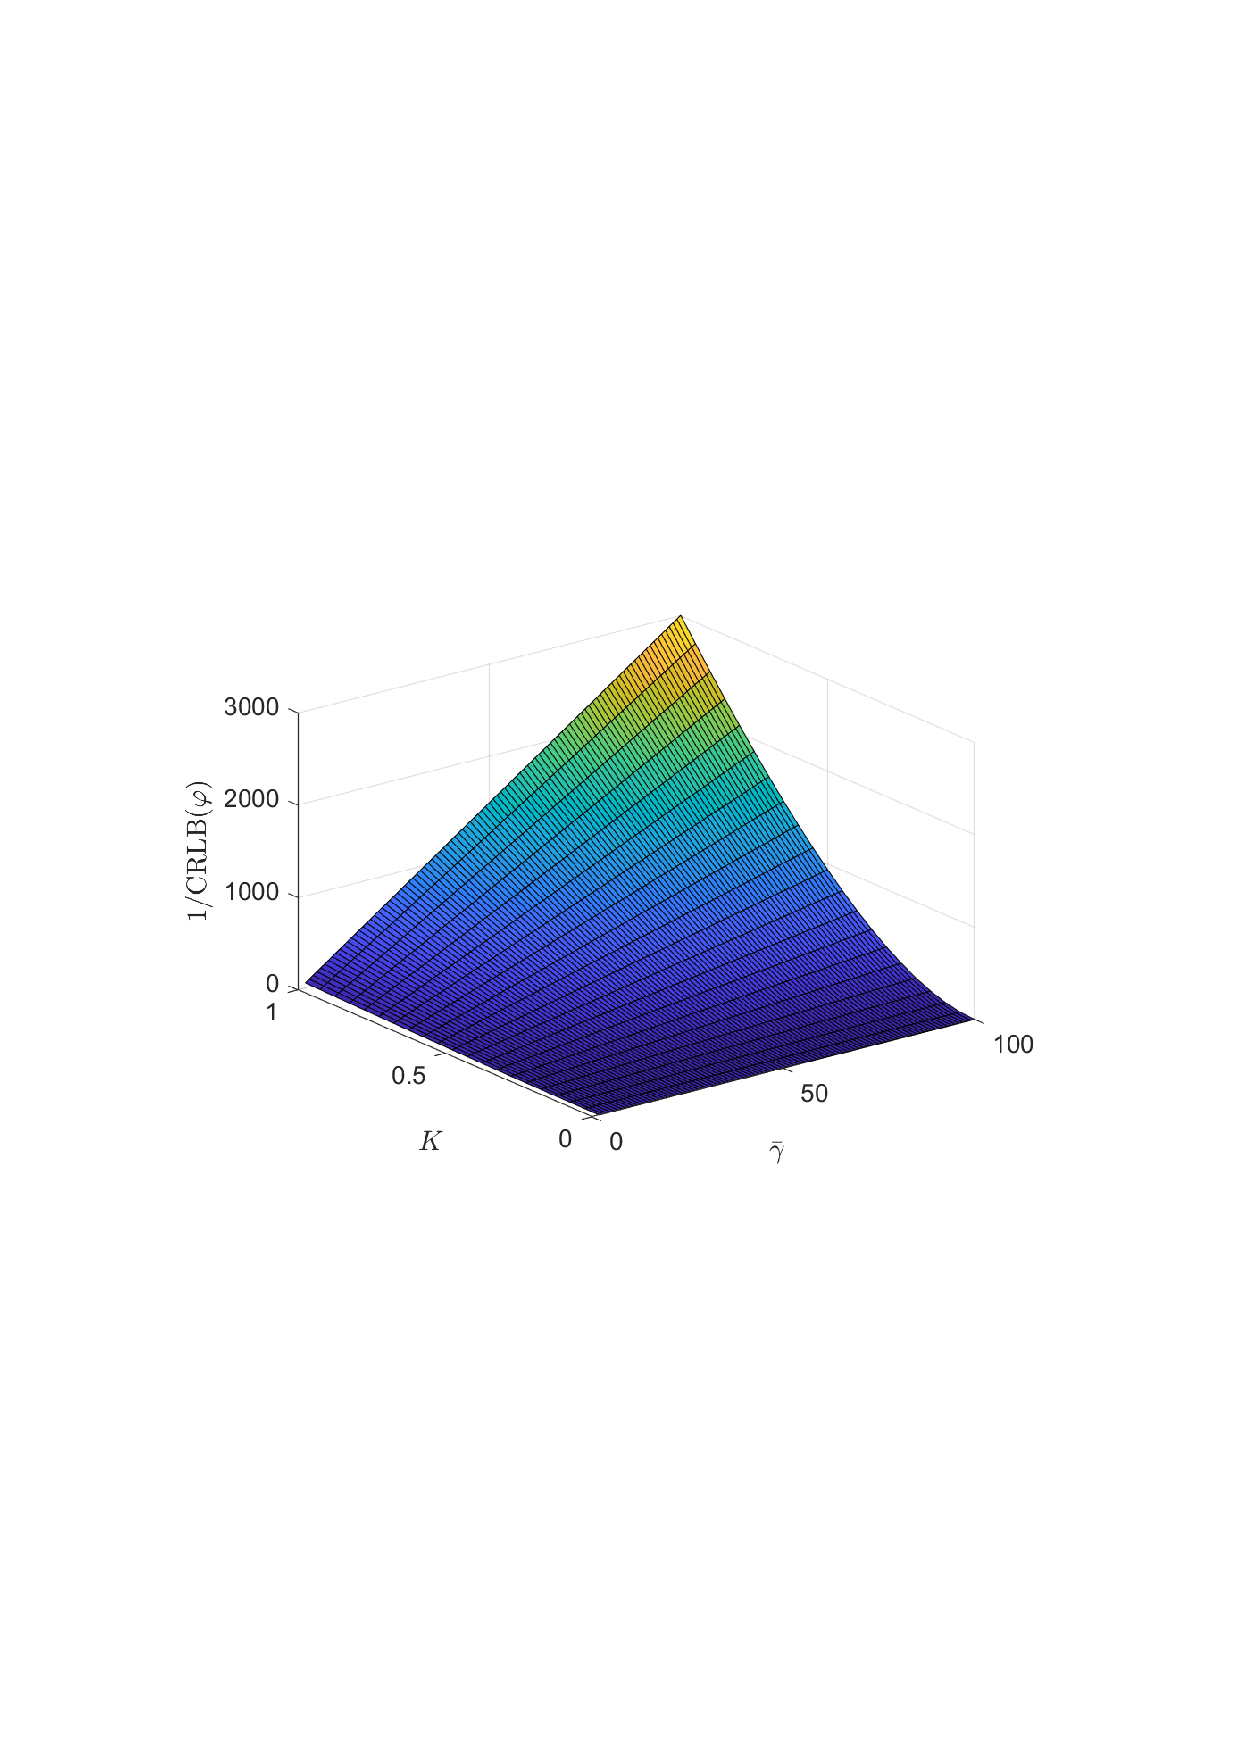
\includegraphics[width=14cm]{figures/crlb.pdf}
        \caption{CRLB}
    \end{figure}

\subsection{von Mises-EM method}
    We discover from our experiments that both the LS method and the Newton-ML method are close to the CRLB. Specifically, the Newton-ML method provides an almost optimal estimator for the phase difference $\varphi$ between the BS-RIS path and the RIS-User path. However, the computation of the Newton-ML estimator is quite complicated due to intensive calculation of modified Bessel functions. Now we introduce an iterative method for estimating $\varphi$ without any computation of special functions.

    This algorithm is based on the Bayesian inference of von-Mises distributions. The von-Mises distribution $VM(\mu, \kappa)$ is a two-parameter distribution on $[0, 2\pi]$, with the probability density function given by 
    \begin{equation}
        p(\theta|\mu, \kappa) = \frac{\exp(\kappa \cos(\theta - \mu))}{2\pi I_0(\kappa)}, 0\leq \theta \leq 2\pi,
    \end{equation}
    where $\mu \in [0,2\pi]$ and $\kappa >0$ being the cyclic location parameter and the concentration parameter. The von-Mises distribution is closely related to the complex Gaussian distribution.
    
    \begin{lemma}[Bayesian estimation of von-Mises distribution]\label{lemma_1}
        Let $\theta \sim \VM(\mu, \kappa)$, and $z \sim \CN(e^{{\rm j}\theta}, \sigma^2)$. Then the posterior distribution $\theta | z$ is also a von-Mises distribution $\VM(\mu', \kappa')$ with parameters $\mu'$ and $\kappa'$ satisfying
        \begin{equation}
            \kappa' e^{{\rm j}\mu'} = \kappa e^{{\rm j}\mu} + \frac{1}{\sigma^2/2}z.
        \end{equation}
    \end{lemma}
    \begin{IEEEproof}
        Since $z=z_r + {\rm j} z_i \sim \CN(e^{{\rm j} \theta}, \sigma^2)$, the conditional density for $z|\theta$ is given by 
        \begin{equation}
            p(z|\theta) = \frac{1}{\sigma^2}\exp\left(-\frac{1}{\sigma^2}\left(\left(z_r - \cos\theta\right)^2 + \left(z_i - \sin\theta\right)^2\right)\right)
        \end{equation}
        The posterior density $p(\theta | z) \propto p(\theta)p(z|\theta)$. Thus
        \begin{equation}
            \begin{aligned}
                p(\theta|z) & \propto \exp(\kappa \cos(\theta - \mu))\exp\left(-\frac{1}{\sigma^2}\left(\left(z_r - \cos\theta\right)^2 + \left(z_i - \sin\theta\right)^2\right)\right) \\
                & \propto \exp\left( \kappa \cos(\theta - \mu) + \frac{2}{\sigma^2}(z_r \cos\theta + z_i\sin\theta) \right) \\
                & \propto \exp\left( \re\left[ \kappa e^{{\rm j} (\theta - \mu)} + \frac{1}{\sigma^2/2}z^{*} e^{{\rm j} \theta} \right] \right) \\
                & = \exp\left( \re\left[ e^{{\rm j} \theta}\left(\kappa e^{-{\rm j}\mu} + \frac{1}{\sigma^2/2} z^*\right)\right] \right).
            \end{aligned}
        \end{equation}
        Since the density of von-Mises distribution $\VM(\mu, \kappa)$ can also be expressed as $p(\theta) \propto \exp\left( \re\left[ e^{{\rm j} \theta}(\kappa e^{{\rm j} \mu})^* \right] \right)$, we can also parameterize the von-Mises distribution by a single complex parameter $\kappa e^{{\rm j}\mu}$. Thus, the above $p(\theta|z)$ is a von-Mises density with parameter $\kappa'e^{{\rm j}\mu'}$, satisfying $\kappa' e^{{\rm j}\mu'} = \kappa e^{{\rm j}\mu} + 1/(\sigma^2/2)\,z$. This completes the proof.
    \end{IEEEproof}
    From the above proof, we can also denote the von-Mises distribution $\VM(\mu, \kappa)$ as $\VM(\kappa e^{{\rm j}\mu})$. This representation is more convenient when manipulating the posterior distributions in Bayesian inference.

    \begin{lemma}[Noncentral $\CN$ posterior distribution on circle is $\VM$]\label{lemma_2}
        Suppose $z \sim \CN(z_0, \sigma^2)$, where $z_0 \in \mathbbm{C}$, and a positive radius $r>0$. Then the posterior distribution of angle $\theta= \arg (z)$ on a circle $|z|=r$ obeys the von-Mises distribution
        \begin{equation}
            p(\theta |\, |z|=r) \sim \VM\left(\arg(z_0), \frac{r|z_0|}{\sigma^2/2}\right).
        \end{equation}
    \end{lemma}
    \begin{IEEEproof}
        Trivial.
    \end{IEEEproof}
    Combining the results of {\bf Lemma \ref{lemma_1}} and {\bf Lemma \ref{lemma_2}}, we can construct the EM algorithm for estimating $\varphi$. Since the output of the power sensors $P[l]$ does not contain phase information, we can treat the phases as latent variables. Let $s_l = \sqrt{P[l]/A}$ be the noisy estimation for $|\alpha + \beta e^{{\rm j} (\varphi + \psi_l)} + v_l|$, and $\theta_l$ be the latent variables $\arg (\alpha + \beta e^{{\rm j} (\varphi + \psi_l)} + v_l)$. Since the noise $v_l \sim {\rm i.i.d.}\;\CN(0, \sigma_v^2)$, then from {\bf Lemma \ref{lemma_2}}, $\theta_l | s_l, \varphi \sim \VM(\arg(\alpha + \beta e^{{\rm j} (\varphi + \psi_l)}), s_l |\alpha + \beta e^{{\rm j} (\varphi + \psi_l)}|/(\sigma_v^2/2))$. Thus, we can infer the latent variables by ML estimation 
    \begin{equation}
        \hat{\theta}_{l, {\rm ML}} | s_l, \varphi = \arg(\alpha + \beta e^{{\rm j} (\varphi + \psi_l)})
        \label{eqn:E-step}
    \end{equation}
    After inferring the latent variables $\hat{\theta}_{l, {\rm ML}}$, we can update the estimation of $\varphi$ using Bayesian rule in {\bf Lemma \ref{lemma_1}}
    \begin{equation}
        \varphi | s_l, \theta_l \sim \VM\left( \kappa e^{{\rm j} \mu} + \frac{1}{\beta\sigma_v^2/2}\sum_{l=0}^{L-1}{\left(s_l e^{{\rm j}\theta_l}-\alpha\right)e^{-{\rm j} \psi_l}}\right)
        \label{eqn:M-step}
    \end{equation}
    Performing E-step with \eqref{eqn:E-step} and M-step with \eqref{eqn:M-step} alternately, then the estimation precision for $\varphi$ can be iteratively improved. Note that although the modified Bessel functions appear in the density function of von-Mises distribution, the bother is avoided in the von Mises-EM algorithm.

    \begin{algorithm}[H] 
        \caption{von Mises-EM phase estimation} \label{alg:VM-EM}
        \setstretch{1.35}
        \begin{algorithmic}[1]
            \REQUIRE Incident wave intensity $\alpha$, $\beta$; sensor data $P[l]$; amplification factor $A$ and noise variance $\sigma_v^2$; predefined phase shifts $\psi_l$.
            \ENSURE $\hat{\varphi}$
            \STATE $s_l \leftarrow \sqrt{P[l]/A}, \forall l=0,1,\cdots,L-1$
            \STATE $\hat{\varphi} \leftarrow \arg\{{\rm FFT}(P)[1]\}$
            \STATE $\kappa \leftarrow 1$
            \WHILE {$\hat{\varphi}$ not convergence}
                \STATE $\mu_l \leftarrow \alpha + \beta e^{{\rm j} (\hat{\varphi}+\psi_l)}, \forall l=0,1,\cdots,L-1$
                \STATE $w_l \leftarrow s_l e^{{\rm j} \arg(\mu_l)} - \alpha, \forall l=0,1,\cdots,L-1$
                \STATE $z_\varphi \leftarrow \kappa e^{{\rm j} \hat{\varphi}} + \left( \sum_{l=0}^{L-1}{w_l e^{-{\rm j} \psi_l}}\right) / (\beta \sigma_v^2/2)$
                \STATE $\hat{\varphi} \leftarrow \arg(z_\varphi)$
                \STATE $\kappa \leftarrow |z_\varphi|$
            \ENDWHILE
        \end{algorithmic}
    \end{algorithm}

    However, in the above {\bf Algorithm \ref{alg:VM-EM}}, we need the interferential parameters $\alpha$ and $\beta$. In fact, these parameters are channel gains that can be directly measured without interference signaling of the BS and UE. 

\subsection{MIMO case: Generalization to Multiusers}

\appendices


\section*{Acknowledgments}

\section*{Appendix A\\ Expectation Evaluation}\label{appendix: expectation evaluation}
    In order to evaluate the expectation $\mathbb{E}[(1-R^2(z_l))P[l]/\lambda_l]$, we first introduce some preliminaries about the noncentral chi distribution $\nc_{\chi_k}(\lambda)$ with noncentrality parameter $\lambda>0$. The distribution $\nc_{\chi_k}(\lambda)$ is the distribution of the length of a $k$-dimensional standard normal distribution $\mathcal{N}({\bm \mu}, {\bm I}_k)$, with $\lambda = \Vert {\bm \mu} \Vert_2$. In particular, we are interested in the case where $k=2$, since that is the case on the complex plane. For  $k=2$, suppose $Y \sim \nc_{\chi_2}(m)$, then
    \begin{equation}
        \mathbb{E}\left[Y\right] = \sqrt{\frac{\pi}{2}}L_{1/2}(-m^2/2),
        \label{eqn:noncentral chi mean}
    \end{equation}
    where $L_{1/2}$ denotes the generalized Laguerre function of order $1/2$. The function $L_{1/2}(x)$ has explicit expression 
    \begin{equation}
        L_{1/2}(x) = e^{x/2}\left[(1-x)I_0\left(-\frac{x}{2}\right)-xI_1\left(-\frac{x}{2}\right) \right].
        \label{eqn:Laguerre half order}
    \end{equation}
    Recall that $x(1-R^2(2\sqrt{x})) \sim \sqrt{x}/2$, the random variable $P[l] \sim a/2 \vert \CN\left((\alpha + \beta e^{{\rm j} (\phi_l + \varphi)})/(\sigma_v / \sqrt{2}), 2\right)\vert^2$, and $\vert \CN\left((\alpha + \beta e^{{\rm j} (\phi_l + \varphi)})/(\sigma_v / \sqrt{2}), 2\right)\vert$ is in fact a noncentral chi distribution of dimension $k=2$ and noncentrality parameter $m=\lvert\alpha + \beta e^{{\rm j} (\phi_l + \varphi)}\rvert/(\sigma_v / \sqrt{2})$ Thus, we can convert the expectation  $\mathbb{E}[(1-R^2(z_l))P[l]/\lambda_l]$ into the expectation of a noncentral chi random variable:
    \begin{equation}
        \begin{aligned}
        \mathbb{E}[(1-R^2(z_l))P[l]/\lambda_l] & = \mathbb{E}\left[\left(1-R^2\left(\frac{\sqrt{\lambda P[l]}}{a/2}\right)\right)\frac{P[l]}{\lambda}\right] \\
        & \approx \left(\frac{a}{\lambda}\right)^2 \mathbb{E}\left[ \sqrt{\frac{\lambda P[l]}{a^2}}/2 \right]\\
        & = \frac{1}{2}\frac{\sqrt{\lambda}}{a}\left(\frac{a}{\lambda}\right)^2 \sqrt{\frac{a}{2}}\mathbb{E}\left[\nc_{\chi_2}(m)\right],\\
        \end{aligned}
        \label{eqn:approx evaluation}
    \end{equation}
    where $m=\lvert\alpha + \beta e^{{\rm j} (\phi_l + \varphi)}\rvert/(\sigma_v / \sqrt{2}) = \sqrt{2\lambda/a} = \sqrt{2\gamma}$, and thus $m^2/2=\gamma$. Plugging \eqref{eqn:noncentral chi mean} and \eqref{eqn:Laguerre half order} into \eqref{eqn:approx evaluation}, we obtain the final expression 
    \begin{equation}
        \begin{aligned}
        \mathbb{E}[(1-R^2(z_l))P[l]/\lambda_l] & \approx \frac{1}{2}\frac{\sqrt{\lambda}}{a}\left(\frac{a}{\lambda}\right)^2 \sqrt{\frac{a}{2}} \sqrt{\frac{\pi}{2}} e^{-\gamma/2}\left[(1+\gamma)I_0(\gamma/2)+\gamma I_1(\gamma/2)\right] \\
        & = \frac{1}{4}\sqrt{\frac{\pi}{\gamma}}e^{-\gamma/2}\left[(1+\gamma^{-1})I_0(\gamma/2)+ I_1(\gamma/2)\right] \\
        & := g(\gamma).
        \end{aligned}
        \label{eqn:approx evaluation result}
    \end{equation}
    The approximation error of the expectation can be upper bounded by the asymptotic expansion error. Assume that the asymptotic expansion error does not exceeds $\delta$, i.e.,
    \begin{equation}
        \lvert x(1-R^2(2\sqrt{x}))-\sqrt{x}/2 \rvert \leq \delta,
        \label{eqn:asymptotic error}
    \end{equation}
    then we have 
    \begin{equation}
        \lvert \mathbb{E}[(1-R^2(z_l))P[l]/\lambda_l] - g(\gamma)\rvert \leq \frac{1}{\gamma^2} \delta. 
    \end{equation}
    We have discovered numerically that $\delta \leq 0.07$, and that as $x\to \infty$, the approximation error tends to zero. Thus, \eqref{eqn:approx evaluation result} is a nearly perfect approximation when $\gamma$ is large. To be more precise, the function $g(\gamma)$ has asymptotic expansion at $\gamma \to +\infty$
    \begin{equation}
        g(\gamma) \sim \frac{1}{2}\left(\frac{1}{\gamma} + \frac{1}{4\gamma^2} + \mathcal{O}(\frac{1}{\gamma^3})\right).
    \end{equation}
    Thus, $1/\gamma - g(\gamma) \sim 1/2\,\Theta(1/\gamma)$, and the relative error of a single term in the CRLB expression is upper bounded by 
    \begin{equation}
        \begin{aligned}
        r & \leq \frac{\delta/\gamma^2}{\lvert \,\lvert 1/\gamma - g(\gamma)\rvert - \lvert g(\gamma) -  \mathbb{E}[(1-R^2(z_l))P[l]/\lambda_l]\rvert\,\rvert} \\
        & \leq \frac{\delta/\gamma^2}{1/((2+\epsilon)\gamma) - \delta/\gamma^2} \\
        & = \frac{\delta}{\gamma/(2+\epsilon) - \delta}, \\
        \end{aligned}
    \end{equation}
    and this upper bound holds whenever $\gamma > (2+\epsilon)\delta$, and $\epsilon$ is chosen to satisfy 
    \begin{equation}
        \frac{1}{\gamma} - g(\gamma) > \frac{1}{(2+\epsilon)\gamma}, \forall \gamma > (2+\epsilon)\delta,
    \end{equation}
    which is equivalent to 
    \begin{equation}
        \epsilon > \frac{1}{1-\gamma g(\gamma)}-2, \forall \gamma > (2+\epsilon)\delta.
    \end{equation}
    Since the function $ 1/(1-\gamma g(\gamma))$ is decreasing on $\gamma>0$, the inequality is equivalent to 
    \begin{equation}
        \epsilon > \frac{1}{1-(2+\epsilon)\delta\, g((2+\epsilon)\delta)}-2.
    \end{equation}
    In fact, choosing $\epsilon=4$ will satisfy all the conditions above when $\delta = 0.07$. So the relative error is upper bounded by 
    \begin{equation}
        r \leq \frac{0.07}{\gamma/6 - 0.07}, \forall \gamma > 0.42.
    \end{equation}
    We can easily see from the above inequality that this approximation becomes arbitrarily good when $\gamma\to\infty$.

\footnotesize
\balance 
\bibliographystyle{IEEEtran}
\bibliography{SensingRIS, IEEEabrv}

\end{document}











